\documentclass[a4paper, 8pt]{extarticle}
\setcounter{page}{0}
\renewcommand{\baselinestretch}{0.92} %spacing between lines

\usepackage{lipsum} %create dummy text

\usepackage{hyperref}

%algorithms
\usepackage{algorithm}
\usepackage[noend]{algpseudocode}

\usepackage[landscape]{geometry}
\geometry{
     %total={210mm,297mm},
     left=2mm,
     right=2mm,
     top=15mm,
     bottom=0mm,
 }
\usepackage[utf8]{inputenc}
\usepackage[normalem]{ulem}

\usepackage{amssymb}
\usepackage{amsmath}
\usepackage{amsfonts}

\usepackage{mathtools}
\usepackage[ngerman]{babel}

\usepackage{multicol} %multiple columns
\usepackage{wrapfig} %wrap text around figures

%get rid of spacing between lists
\usepackage{enumitem} 
    \setlist{nolistsep}

%imagepackage
\usepackage{graphicx} 
    \graphicspath{ {./images/} }

\usepackage{parskip} %Einzug aus, Absatzabstand ein
    \tolerance=2000 %Toleranz für Wortzwischenräume
    \setlength{\emergencystretch}{20pt} %Zusätzliche Zeilendehnbarkeit in Notfällen
    \setlength\parindent{0pt}
    \setlength{\columnseprule}{1px} %thickness of column seperator

%New Titles
\usepackage{tcolorbox}
    \definecolor{seccol}{RGB}{7, 61, 50}
    \definecolor{subseccol}{RGB}{29, 120, 116}
    \definecolor{subsubseccol}{RGB}{103, 146, 137}

\usepackage[explicit]{titlesec}

\titleformat{\section}
  {\normalfont\bfseries}
  {}
  {0em}
  {\pgfsetfillopacity{1}
    \colorbox{seccol}{
        \parbox{\dimexpr\linewidth-4.5\fboxsep\relax}{
            \textcolor{white}{\thesection\quad#1}}}
    \pgfsetfillopacity{1}}
  
\titleformat{\subsection}
  {\normalfont\bfseries}
  {}
  {0em}
  {\pgfsetfillopacity{1}
    \colorbox{subseccol}{
        \parbox{\dimexpr\linewidth-4.5\fboxsep\relax}{
            \textcolor{white}{\thesubsection\quad#1:}}}
    \pgfsetfillopacity{1}}

\titleformat{\subsubsection}
  {\normalfont\bfseries}
  {}
  {0em}
  {\pgfsetfillopacity{1}
    \colorbox{subsubseccol}{
        \parbox{\dimexpr\linewidth-4.5\fboxsep\relax}
            {\textcolor{white}{\thesubsubsection\quad#1:}}}
    \pgfsetfillopacity{1}}
    
\titlespacing{\section}{0pt}{\parskip}{-0.75\parskip}    
\titlespacing{\subsection}{0pt}{\parskip}{-0.75\parskip}
\titlespacing{\subsubsection}{0pt}{\parskip}{-0.75\parskip}

%custom header with title & authors
\usepackage{fancyhdr} 
    \pagestyle{fancy}
    \fancyhf{}
    \rhead{Joshua Näf, \textit{naefjo@ethz.ch}}
    \chead{\textbf{\thepage}}
    \lhead{\textbf{MAD 1 Spring 20 Dr. J. Walther}}
    \setlength{\headsep}{1mm}


%colourful boxes for math mode
% Syntax: \colorboxed[<color model>]{<color specification>}{<math formula>}
\usepackage{xcolor}
\newcommand*{\colorboxed}{}
\def\colorboxed#1#{%
  \colorboxedAux{#1}%
}
\newcommand*{\colorboxedAux}[3]{%
  % #1: optional argument for color model
  % #2: color specification
  % #3: formula
  \begingroup
    \colorlet{cb@saved}{.}%
    \color#1{#2}%
    \boxed{%
      \color{cb@saved}%
      #3%
    }%
  \endgroup
}    


%TODO command    
\newcommand{\TODO}[1]{\large\textcolor{red}{\textbf{TODO: #1\\}}\normalsize}

% Define new command for varphi
\newcommand{\p}{\varphi}
\newcommand{\w}{\textbf{\textit{w}}}
\newcommand{\y}{\textbf{\textit{y}}}    
\renewcommand{\Vec}[1]{\textbf{\textit{#1}}}
    
    
\title{MAD 1 Summary}
\author{Joshua Näf}
\date{}

\begin{document}

\maketitle
\begin{center}
MAD 1 Summary created by \href{mailto:naefjo@ethz.ch}{\textit{naefjo@ethz.ch}}\\
\parbox{0.5\linewidth}{
\begin{center}
This summary has been written based on the Lecture 151-0431-00L Models, Algorithms and Data: Introduction to Computing by Dr. Jens Honoré Walther and Dr. Georgios Arampatzis (Spring 20). There is no guarantee for completeness and/or correctness regarding the content of this summary. Use it at your own discretion

Source Code: \url{https://github.com/naefjo/MAD-1-Summary}
\end{center}
}
\end{center}
\newpage

\begin{center}
    \begin{multicols*}{2}
        \tableofcontents
    \end{multicols*}
\end{center}

\begin{multicols*}{4}

\section{Linear Least Squares}
    \subsection{Parametric Function Fitting}
    For $A \in\mathbb{R}^{N \times M}$: \textit{Null Space} or \textit{Kernel} = subspace of all vectors $\mathbf{x}\in\mathbb{R}^N$ s.t. $A\mathbf{x}=0$. It is denoted by null($A$). \textit{Left Null Space} or \textit{Cokernel}: null($A^\top$). \textit{Column Space} or \textit{Range} or \textit{Image} of $A$ is the space spanned by the columns of A and is denoted by range($A$). \textit{Row Space} or \textit{Coimage} of $A$: range($A^\top$).
    
    We want to minimize error:
    \begin{equation*}
        \|\mathbf{e}\|_2=\sqrt{\sum_{i=1}^N e_i^2}=\sqrt{\sum_{i=1}^N (y_i-f(x_i))^2}
    \end{equation*}
    Choosing different norms yields different results.
    
    \textbf{N: \#Data Points \\M: \#Free Parameters/Functions}

\subsection{Linear Least Squares}
    Fit data $\left\{(x_i, y_i)\right\}_{i=1}^{N}$ with a function $f(x)$ which can be expressed as M linearly independent functions $\p_k(x)$,
    \begin{equation*}
        f(x;\textbf{\textit{w}}) = \sum_{k=1}^M w_k\p_k(x)
    \end{equation*}
    where $\textbf{\textit{w}}=(w_1, w_2, \dots, w_M)$ are the unknown weights.
    Functions can be nonlinear but \textbf{weights have to enter lineraly}.
    
    Goal: find \textbf{\textit{w}} s.t. error $E(\textbf{\textit{w}}) = \|\mathbf{e(\textbf{\textit{w}})}\|^2_2$ is minimised.
    \begin{equation*}
        \textbf{\textit{w}}^\star = \underset{\textbf{\textit{w}}}{\arg\min}\textrm{ } E(\textbf{\textit{w}})\Rightarrow \frac{d E(\textbf{\textit{w}})}{d \textbf{\textit{w}}} = 0
    \end{equation*}
    Matrix notation leads us to: $A\Vec{w}= \Vec{y}$
    \\$A\in\mathbb{R}^{N\times M}$, $\textbf{\textit{w}}\in\mathbb{R}^{M}$, $\textbf{\textit{y}}\in\mathbb{R}^{N}$
    \begin{equation*}
        \begin{bmatrix}
            \p_1(x_1) & \p_2(x_1) & \dots & \p_M(x_1)\\
            \p_1(x_2) & \p_2(x_2) & \dots & \p_M(x_2)\\
            \vdots & \ddots & & \vdots\\
            \vdots & & \ddots & \vdots\\
            \p_1(x_N) & \p_2(x_N) & \dots & \p_M(x_N)\\
        \end{bmatrix}
        \begin{bmatrix}
            w_1\\
            w_2\\
            \vdots\\
            w_M
        \end{bmatrix}
        = 
        \begin{bmatrix}
            y1\\
            y_2\\
            \vdots\\
            \vdots\\
            y_N
        \end{bmatrix}
    \end{equation*}
    \begin{itemize}
        \item M=N there exists unique solution $\textbf{\textit{w}} = A^{-1}\textbf{\textit{y}}$.
        \item M\textgreater N System is underdetermined and has infinitely many solutions
        \item M\textless N System is overdetermined. We can approximate a solution $A\textbf{\textit{w}}\approx \textbf{\textit{y}}$ with least squares requiring $E(\textbf{\textit{w}}) = \|\textbf{\textit{y}}-A\textbf{\textit{w}}\|_2^2$ be minimal.
    \end{itemize}
    \begin{equation*}
        \colorboxed{red}{
            \w^\star = (A^\top A)^{-1}A^\top\y
        }
    \end{equation*}
    
    \subsubsection{Solution for Linear Functions}
        Consider set of data $\{x_i, y_i\}_{i = 1}^N$ which we want to fit to $y = w_1 + w_2 x$
        \begin{equation*}
        \begin{bmatrix}
            1 & x_1\\
            1 & x_2\\
            \vdots & \vdots\\
            1 & x_N\\
        \end{bmatrix}
        \begin{bmatrix}
            w_1\\
            w_2\\
        \end{bmatrix}
        = 
        \begin{bmatrix}
            y1\\
            y_2\\
            \vdots\\
            y_N
        \end{bmatrix}
    \end{equation*}
    % \begin{equation*}
    %     \begin{bmatrix}
    %         N & \sum_{i=1}^N x_i\\
    %         \sum_{i=1}^N x_i & \sum_{i=1}^N x_i^2
    %     \end{bmatrix}
    %     \begin{bmatrix}
    %         w_1\\
    %         w_2\\
    %     \end{bmatrix}
    %     =
    %      \begin{bmatrix}
    %         \sum_{i=1}^N y_i\\
    %         \sum_{i=1}^N x_iy_i
    %     \end{bmatrix}
    % \end{equation*}
    \begin{equation*}
        w_1^\star = \frac{\sum_{i=1}^N x_i^2\sum_{i=1}^N y_i-\sum_{i=1}^N x_i\sum_{i=1}^N x_iy_i}{N\sum_{i=1}^N x_i^2-\left(\sum_{i=1}^N x_i\right)^2}
    \end{equation*}
    \begin{equation*}
        w_2^\star = \frac{N\sum_{i=1}^N x_iy_i-\sum_{i=1}^N x_i\sum_{i=1}^N y_i}{N\sum_{i=1}^N x_i^2-\left(\sum_{i=1}^N x_i\right)^2}
    \end{equation*}

    \subsubsection{Orthonormal Case}
        Let $\mathbf{a}_i$ be the columns of $A \in\mathbb{R}^{N\times M}$. Columns are orthogonal iff \begin{equation*}
            \mathbf{a}_i \cdot \mathbf{a}_j = \delta_{ij} \quad 1 \leq i,j \leq M
        \end{equation*}
        An \textit{orthogonal Matrix} has the following properties:
        \begin{equation*}
            A^\top = A^{-1}; \qquad \|A\mathbf{u}\| = \|\mathbf{u}\|
        \end{equation*}
        LSQ simplifies to:
        \begin{equation*}
            \textbf{\textit{w}}^\star = A^\top\textbf{\textit{y}}
        \end{equation*}
        % \TODO{example?}
        
    \subsection{Geometric Interpretation}
        The columns of A span a M-dimensionl space. The least squares method finds the solution $\w^\star$ s.t. $A\w^\star$ ist the projection of $\y$ on the column space of $A$.
        We observe that the residual $\mathbf{e} = \mathbf{y}-A\w^\star$ is perpendicular to  range($A$) and has minimal 2-norm ($\|e\|=\|\y-A\w\|$ is minimal for $\w = \w^\star$)
        \begin{center}
            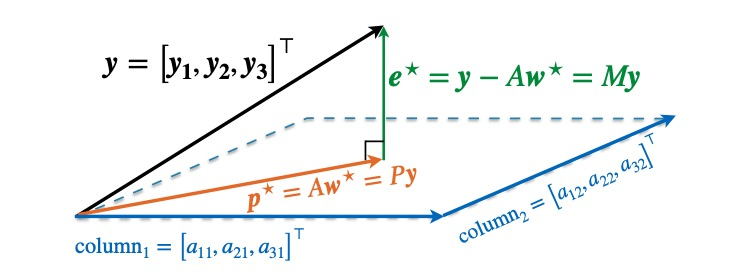
\includegraphics[width = 0.7\linewidth]{images/01/geometric_interpretation.jpg}\\
            Geometric interpretation for $N=3$ and $M = 2$
        \end{center}
        
        $\mathbf{e}^\star\in$ left nullspace $A$
        
        $A\w = \y$ has a solution iff $\y\in$ range $A$ $\Rightarrow \mathbf{e} = 0$
        \subsubsection{Projection Matrix P}
            closest point to $\y$ is $\Vec{p} = A\w^\star = P\Vec{y}$
            \begin{equation*}
                \colorboxed{red}{
                    P = A(A^\top A)^{-1}A^\top
                }
            \end{equation*}
            P is called a \textit{projection matrix} and has the following properties:
            \begin{equation*}
                P = P^\top \textrm{ (symmetric)}; \quad P^2 = P \textrm{ (idemptotent)}
            \end{equation*}
            
            We can write the error as $\Vec{e} = \y - A\w^\star =\y -P\y = M\y$
            \begin{equation*}
                M = \mathbb{I} - A(A^\top A)^{-1}A^\top
            \end{equation*}
            where $M$ is also a projection matrix, projecting onto null($A^\top$) (space orthogonal to the column space of $A$), whereas P projects onto range($A$)
            \begin{equation*}
                P + M = \mathbb{I}; \quad PM=0; \quad PA=A; \quad MA=0
            \end{equation*}
        

    \subsection{Numerical Solutions}
    \subsubsection{Condition Number}
        Numerical solution is affected by round-off error. we define $\delta\w = \w -\Tilde{\w}$ and $\delta\y = \y -\Tilde{\y}$ where $\Tilde{\w},\Tilde{\y}$ are the numerical solutions to LSQ and $A\Tilde{\w} = \Tilde{\y}$.
        
        \textit{If $\|\delta\y\|$ is small is $\|\delta\w\|$ small as well?} $\Rightarrow$ No.
        
        Condition number:
        \begin{equation*}
            \colorboxed{red}{
                \kappa(A)=\|A\|\|A^{-1}\|
            } 
            \qquad \kappa(A)\in[0,\infty)
        \end{equation*}
        We call a problem \textit{well defined} if $\kappa(A)$ is not too large. In that case the computed solution will be close to the true solution.
        
        Interpretation: \textit{How close a Matrix is to being singular.}
        
        Orthogonal Matrices: $\kappa(A)=1$
        
        $\|A\|_2 = \sqrt{\rho(A^\top A)}$ where $\rho$ is the largest Eigenvalue
        
        $\kappa_2(A^\top A) = \kappa_2(A)^2 \Rightarrow$ bad for LSQ
        
    \subsubsection{QR decomposition}
        $Q\in\mathbb{R}^{N\times N}$ is orthogonal and $Q_1\in\mathbb{R}^{N\times M}$ is a matrix with orthogonal columns and $R_1\in\mathbb{R}^{M \times M}$ is upper triangle and invertible.
        \begin{equation*}
            \colorboxed{red}{
                A =\underbrace{\begin{bmatrix} Q_1 & Q_2 \end{bmatrix}}_Q \underbrace{\begin{bmatrix} R_1 \\ 0 \end{bmatrix}}_R = Q_1 R_1
            } \
            \colorboxed{red}{
                \w = R_1^{-1}Q_1^\top \y
            }
        \end{equation*}
        $R_1$ is upper triangle $\rightarrow$ \textbf{no need to compute inverse}, just solve the Linear SoE 
        \begin{equation*}
            R_1\w=Q_1^\top\y,\quad 
            \textnormal{with: }\|R_1\|=\|R_1 Q_1\| = \|A\|
        \end{equation*}
        Condition of the matrices involved in the solution is the same as the condition of $A$
        
    \subsubsection{Singular Value Decomposition (SVD)}    
        The SVD of a Matrix $A\in\mathbb{R}^{N\times M}$ with $\textrm{rank}(A) = \rho$ decomposed $A$ as,
        \begin{equation*}
            A = \begin{bmatrix} U_r & U_n \end{bmatrix} \begin{bmatrix} S & 0 \\ 0 & 0 \end{bmatrix} \begin{bmatrix}V_r^\top \\ V_n^\top \end{bmatrix} = U\Sigma V^\top
        \end{equation*}
        $U\in\mathbb{R}^{N\times N}$ and $V\in\mathbb{R}^{M\times M}$ are orthogonal matrices. $\Sigma\in\mathbb{R}^{N\times M}$ is a diagonal matrix and
        $S = \textrm{diag}(\sigma_1,\dots,\sigma_\rho)$ where $\sigma_1 \geq \sigma_2 \geq \dots \sigma_\rho \geq 0$ with $\sigma_i$ being the \textit{singular values} of $A$.
        \begin{equation*}
            \Sigma^+ = \begin{bmatrix} S^{-1} & 0\\ 0 & 0 \end{bmatrix}
        \end{equation*}
        \textit{Moore-Penrose Pesudoinverse:}
        \begin{gather*}
            A^+ = (A^\top A)^{-1}A^\top,\quad
            \colorboxed{red}{
             A^+ = V\Sigma^+ U^\top
            }\\
            \colorboxed{red}{
                \w^\star = V\Sigma^+ U^\top \y
            }
        \end{gather*}
        $\Rightarrow\Sigma V^\top\w^\star = U^\top\y$ and $\kappa(\Sigma V^\top) = \kappa(A)$

\section{Nonlinear Systems}
    \subsection{Root Finding Problem}
    Every nonlinear equation $g(x) = h(x)$ can be written as $g(x) - h(x) = f(x) = 0$ $\Rightarrow$ We transform the problem into a root finding problem for $f(x)$: find $x^\star$ s.t.
    \begin{equation*}
        \colorboxed{red}{
        \begin{aligned}
            f(x^\star) &= 0\\
            e_k = x_k -x^\star &\ \big(\approx x_k -x_{k-1}\big)
        \end{aligned}
        }
    \end{equation*}
    There is no general formula to find a root of a nonlinear function $\rightarrow$ iterative methods that, from an initial guess $x_0$, produce a sequence $x_0, x_1, \dots, x_k$ that converges to $x^\star$ for $k\to\infty$.
    
    % \subsubsection{Existence of a root}
    %     \begin{itemize}
    %         \item \textit{Intermediate Value Theorem:} If $f$ continuous on $[a,b]$, $\exists x^\star$ s.t. $f(x^\star)=y$ $ \forall y\in [f(a),f(b)]$
    %         \item \textit{Bolzano's Theorem:} If $f$ continuous on $[a,b]$ and $\textrm{sign}(f(a)) \neq \textrm{sign}(f(b))$, $\exists x^\star$ s.t. $f(x^\star)=0$
    %     \end{itemize}
        
    \subsubsection{Sensitivity and Conditioning}
        \textit{If $|f(\Tilde{x})|\approx 0$ does this mean that $|\Tilde{x}-x^\star|\approx0$?}
        We call a system ($f$) \textbf{well-conditioned} when a small change in input causes a small change in the output. \textbf{Ill-conditioned} if small change in input causes a large change in output.
        
        Condition number of root finding problem:
        \begin{equation*}
            \colorboxed{red}{
                \kappa = \frac{1}{|f'(x^\star)|}
            }
        \end{equation*}
        
        If $f'(x)=0$ the problem is ill-conditioned. This is the case for roots with \textbf{multiplicity m} $> 1$.
        
        \subsubsection{Order of Convergence}
            We want the sequence $\{x_k\}_{K=0}^{\infty}$ to converge to $x^\star$ as quick as possible. In order to quantify "\textit{fast}" we define the order of convergende as
            \begin{equation*}
                \lim_{k\to\infty}\frac{|e_{k+1}|}{|e_k|^r}= C
            \end{equation*}
            \textbf{order of convergence} $r$ and \textbf{rate of convergence} $C$
            \begin{itemize}
                \item $r=1$: if $C\in(0,1)$ linear convergence. If $C = 0$ superlinear, $C = 1$ sublinear
                \item $r=2$: quadratic convergence
            \end{itemize}{}

\subsection{Bisection Method}
    \begin{center}
        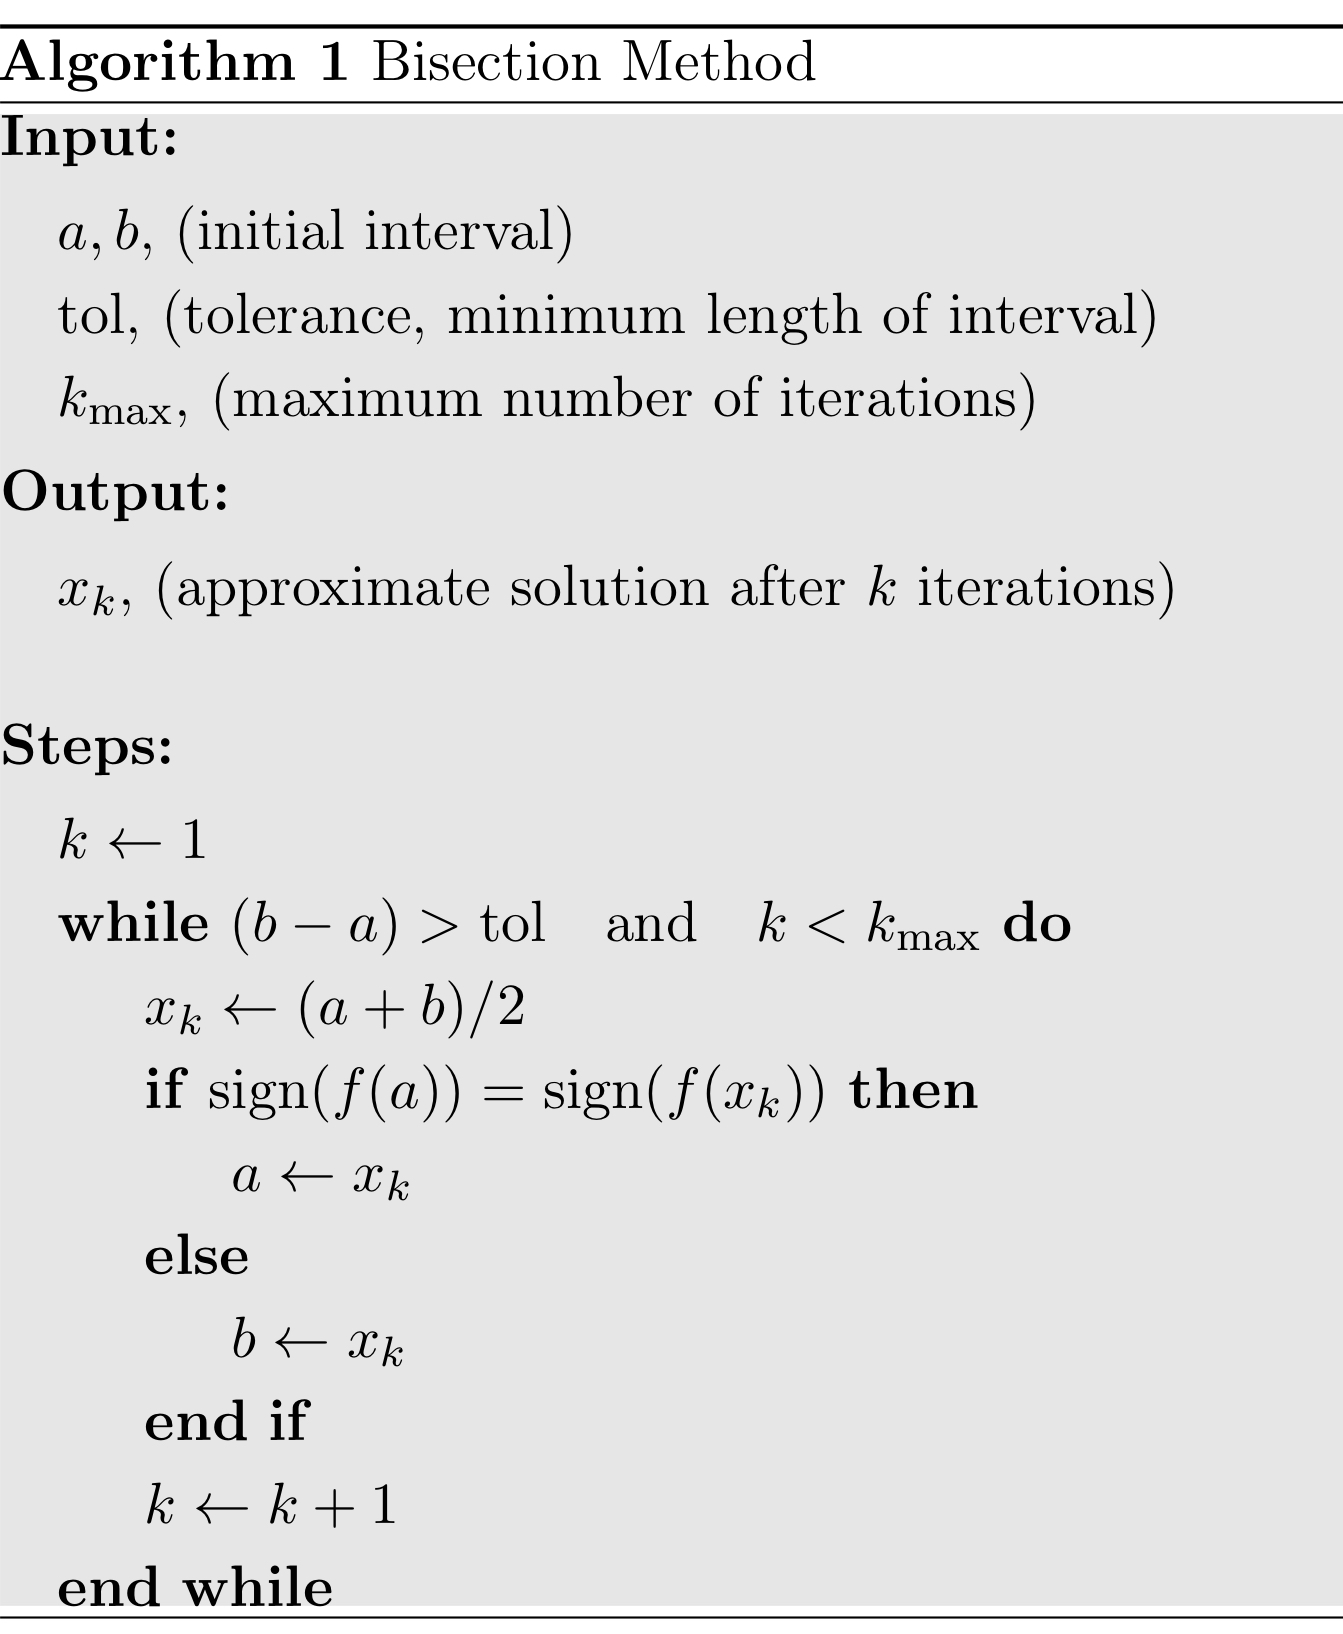
\includegraphics[width=0.9\linewidth, height = 50mm]{images/02/bisection.jpeg}
    \end{center}
    Order of convergence: 1 and rate of convergence. $1/2$
    
    Require number of iterations $k$ to achieve tequired tolerance tol.
    \begin{equation*}
        |e_k| = \textrm{tol} \Rightarrow \frac{b-a}{2^k}=\textrm{tol} \Rightarrow k = \log_2\left(\frac{b-a}{\textrm{tol}}\right)
    \end{equation*}
    \textbf{Advantages:}
    \begin{itemize}
        \item Certain to converge
        \item Only requires signs and not function values
        \item $f$ does not need to be differentiable only continuous
    \end{itemize}
    
    \textbf{Disadvantages:}
    \begin{itemize}
        \item Convergence is slow
        \item Initial interval needs to be known beforehand
        \item Cant be easily generalized to higher dimensions
    \end{itemize}



\subsection{Newtons Method}
    Function $f$ continuous and differentiable at $x^\star$.
    \begin{equation*}
        \colorboxed{red}{x_{k+1} = x_k - \frac{f(x_k)}{f'(x_k)}} \ \underbrace{x_{k+1} = x_k - m\frac{f(x_k)}{f'(x_k)}}_{\textnormal{roots with multiplicity }m>1}
    \end{equation*}
    \textbf{Advantages:}
    \begin{itemize}
        \item Quadratic convergence
    \end{itemize}
    
    Newtons method converges quadratically if:
    \begin{equation*}
        \lim_{k\to\infty}\frac{|e_{k+1}|}{|e_k|^2} = \lim_{k\to\infty}\frac{|f''(\xi_k|)}{2|f'(x_k)|}=\frac{|f''(x^\star)|}{2|f'(x^\star)|}=C<\infty
    \end{equation*}
    
    \textbf{Disadvantages:}
    \begin{itemize}
        \item Small changes in IV may change root
        \item\textbf{Root with multiplicity $m>1$ convergence rate only linear}
        \item Not guaranteed to converge
        \item if $f'(x_k)=0$ for some $k$ we cannot proceed
        \item requires evaluation of both $f(x_k)$ and $f'(x_k)$
    \end{itemize}
    \begin{center}
    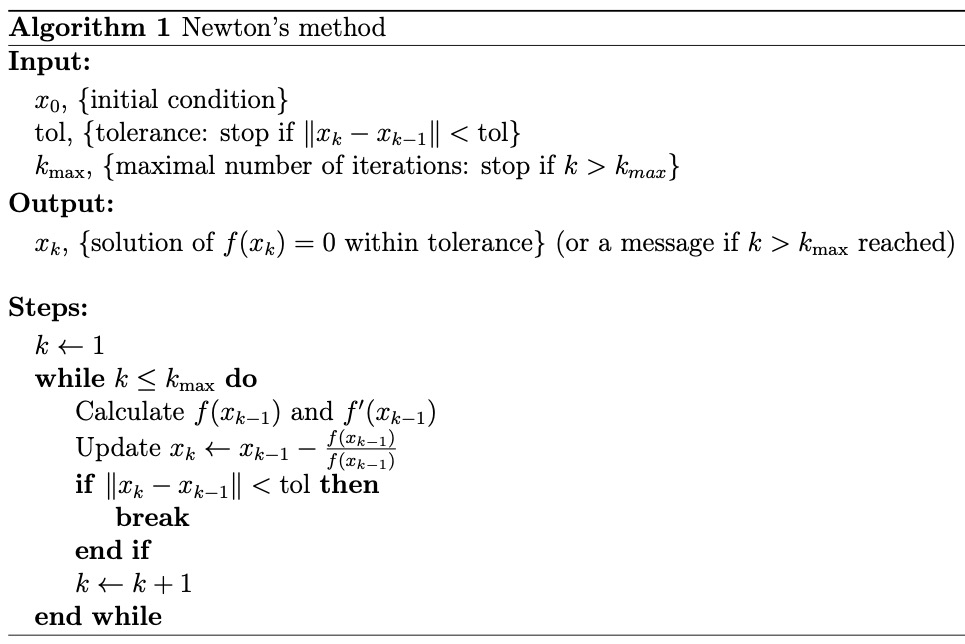
\includegraphics[width=\linewidth]{images/02/newtons_method.jpg} 
    \end{center}
    
\subsection{Secant Method}
    Modification of Newtons method by approximating $f'(x_k) \approx \frac{f(x_k)-f(x_{k-1})}{x_k-x_{k-1}}$
    \begin{equation*}
        \colorboxed{red}{x_{k+1} = x_k - f(x_k)\frac{x_k-x_{k-1}}{f(x_k)-f(x_{k-1})}}
    \end{equation*}
    Order of convergence: $\varphi = \frac{1+\sqrt{5}}{2} \approx 1.618$ (simple roots).
    
    \textbf{Advantages:}
    \begin{itemize}
        \item Avoid evaluation of derivative
        \item Only one function evaluation at each step
    \end{itemize}
    \textbf{Disadvantages:}
    \begin{itemize}
        \item Convergence rate is not quadratic
        \item Needs two initial approximations
    \end{itemize}
    
\subsection{Numerical Computation of the Order of Convergence}
    Compute the error $e_k = x_k-x^\star \, \forall k$ for a function with known root $x^\star$. Then, evaluate the convergence rate $r_k$ as a sequence which will converge to the theoretical $r$.
    \begin{equation*}
        \colorboxed{red}{r \approx \frac{\log\left|\frac{e_{k+2}}{e_{k+1}}\right|}{\log\left|\frac{e_{k+1}}{e_{k}}\right|}} \ \textnormal{log base 10}
    \end{equation*}


    \section{Sets of equations}
    General systems of $N$ non-linear functions $f_i(\Vec{x})$, $i=1,\dots,N$, where $\Vec{x}= (x_1, \dots, x_M)^\top$ is a vector of $M$ unknowns. Find $\Vec{x}^\star$, st. $\colorboxed{red}{f_i(\Vec{x}^\star) = 0 \quad i = 1,\dots,M}$
    
    We define the \textit{Jacobian Matrix} $J(\Vec{x})$ with elements $J_{ij}(\Vec{x}) = \frac{\partial f_i(\Vec{x})}{\partial x_j}$
    \begin{equation*}
        J(\Vec{x}) = 
        \begin{bmatrix}
            \frac{\partial f_1(\Vec{x})}{\partial x_1} & \frac{\partial f_1(\Vec{x})}{\partial x_2} & \dots & \frac{\partial f_1(\Vec{x})}{\partial x_M}\\
            \frac{\partial f_2(\Vec{x})}{\partial x_1} & \frac{\partial f_2(\Vec{x})}{\partial x_2} & \dots & \frac{\partial f_2(\Vec{x})}{\partial x_M}\\
            \vdots & \vdots & \ddots & \vdots\\
            \frac{\partial f_N(\Vec{x})}{\partial x_1} & \frac{\partial f_N(\Vec{x})}{\partial x_2} & \dots &  \frac{\partial f_N(\Vec{x})}{\partial x_M}
        \end{bmatrix}
    \end{equation*}
    
    \subsection{Condition Number}
        For a system of $N$ non-linear equations and $M$ unknowns the condition number of the root finding problem for the root $\Vec{x}^\star$ of $F$ is $\|J^{-1}(\Vec{x}^\star)\|$
    
    \subsubsection{Newtons Method}
    If we set $\Vec{x}_{k+1} = \Vec{x}_k + \Vec{z}$ we have to solve $A\Vec{z} = \Vec{b}$ at every step with $A = J(\Vec{x}_k)$ and $\Vec{b} = -F(\Vec{x}_k)$
    \begin{gather*}
        \mathbf{0}=F(\Vec{x}^\star) \approx F(\Vec{x}_k) + J(\Vec{x}_k)(\Vec{x}^\star -\Vec{x}_k)\\
        J(\Vec{x}_k)(\Vec{x}_{k+1} - \Vec{x}_k) = -F(\Vec{x}_k)
    \end{gather*}
    
    \textbf{Netwon-Raphson Method (\textit{N}=\textit{M}):}
    \begin{equation*}
        \colorboxed{red}{\Vec{x}_{k+1} = \Vec{x}_k - J^{-1}(\Vec{x}_k)F(\Vec{x}_k)}
    \end{equation*}
    We do not invert $J(\Vec{x}_k)$ but solve $J(\Vec{x}_k)\Vec{z} = -F(\Vec{x}_k)$ for $\Vec{z}$ and update $\Vec{x}_{k+1} = \Vec{x}_k + \Vec{z}$
    
    Provided that the Jacobian is not singular the convergence rate is quadratic.
    
    \textbf{Pseudo-Newton Method (\textit{N}$\neq$\textit{M}):}
    \begin{equation*}
        \colorboxed{red}{\Vec{x}_{k+1} = \Vec{x}_k - J^{+}(\Vec{x}_k)F(\Vec{x}_k)}
    \end{equation*}
    Assuming J always has full rank
    
    \begin{center}
        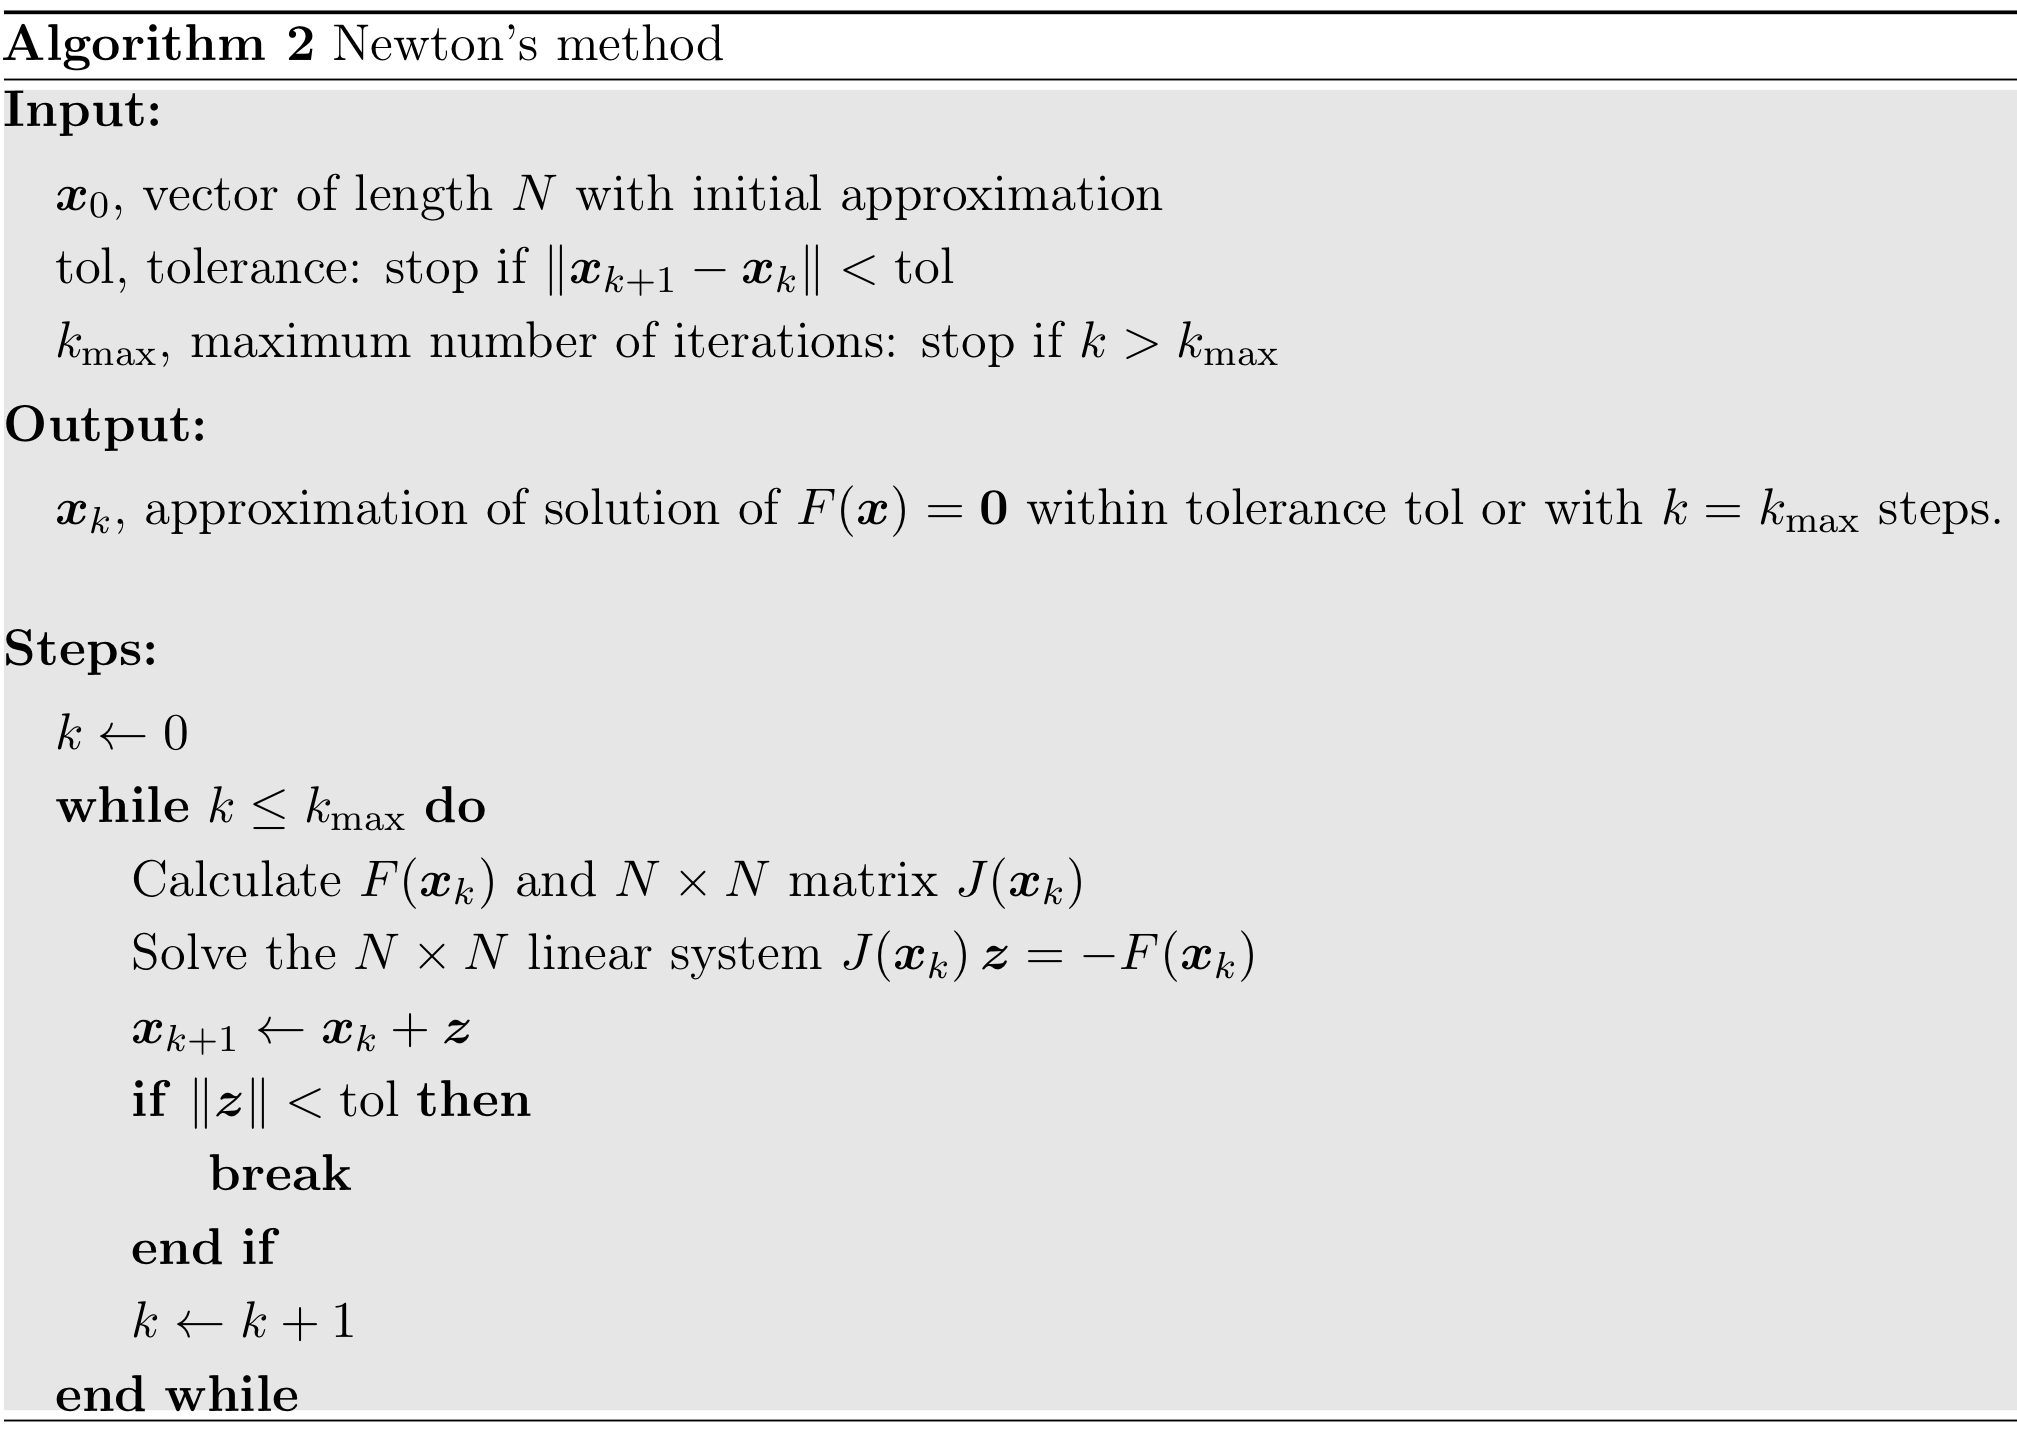
\includegraphics[width = \linewidth]{images/02/soe_newtons_meth.jpeg}
    \end{center}
    \subsection{Non-Linear Optimization}
    Find $\Vec{x}^\star = \underset{\Vec{x}}{\arg\min} \textrm{ }E(\Vec{x})$ with $E:\mathbb{R}^M\rightarrow \mathbb{R}$
    \\Maximizing $E(\Vec{x})$ $\Leftrightarrow$ minimizing $-E(\Vec{x})$
    
    Sufficient condition for a crit point $\Vec{x}^\star$ is $\nabla E(\Vec{x}^\star) = 0$
    \subsubsection{Newtons Method/Update Rule}
    $F(\Vec{x}) = \nabla E(\Vec{x}) \overset{!}{=} 0\rightarrow$minimization problem to a root finding problem.
    \begin{gather*}
        J(\Vec{x}) = \nabla^2E(\Vec{x}) \
        \colorboxed{red}{
        \begin{aligned}
            \nabla^2E(\Vec{x}_k)\Vec{z} &= -\nabla E(\Vec{x}_k)\\
            \Vec{x}_{k+1} &= \Vec{x}_k + \Vec{z}
        \end{aligned}
        }
    \end{gather*}
    
    
\section{Inter- and Extrapolation}
    \subsection{Lagrange Interpolation}
    We want a base polynomial which satisfies $l_i(x_j) = \delta_{ij}$. Create a function of order $N-1$ which perfectly fits $N$ data points.
    \begin{equation*}
        \underbrace{\colorboxed{red}{\ell_k(x) = \prod_{\substack{i=1 \\ i \neq k}}^N \frac{x-x_i}{x_k-x_i}
        }}_{\textnormal{Lagrange Functions}}
        \,
        \underbrace{\colorboxed{red}{
        f(x)=\sum_{k=1}^N y_k \ell_k(x)
        }}_{\textnormal{Lagrange Interpolator}}
    \end{equation*}
    
   
    
    \subsubsection{LSQ vs Interpolation}
        \textbf{Noise:} LSQ robust to noise. Interpolation passes exactly through $(x_i,y_i)\forall i$.
        \textbf{Note:} Lagrange function is dependant ond $x_i$ only.
        
        \textbf{Data points:} Terms of higher order than order of data cancel out in the Lagrange interpolator. I.e. if data linear but 5 data points, lagrange will still be linear. \textbf{LSQ also robust to few data points.}
        
        \textbf{Stability:} Hard to approx. loc. behaviour if interpolator used as global function. Oscillatory behaviour at the endpoints (higher order). Fluctuations in one region may affect the function over the whole domain.
        % LSQ better than Interpolation since Interpolation will pass exactly through the points and take noise into account whereas LSQ is robust to noise. 
    \subsection{Cubic Splines}
    Idea: split interval into subdomains and the construct a piecewise approximation in each subdomain. Cubic functions will lead to piecewise linear $f''$.
    
    Data: $\{x_i,y_i\}_{i=1,\dots,N}$ Let $f_i(x)$ be a cubic function in between $x_i < x < x_{i+1}$
    \begin{equation*}
    \colorboxed{red}{
    \begin{aligned}
        \frac{\Delta_{i-1}}{6}f_{i-1}'' + \left(\frac{\Delta_{i-1}+\Delta_i}{3}\right)f_i'' + \frac{\Delta_i}{6}f''_{i+1} \\= \frac{y_{i+1}-y_i}{\Delta_i} - \frac{y_i-y_{i-1}}{\Delta_{i-1}}
    \end{aligned}
    }
    \end{equation*}
    where $\Delta_i = x_{i+1}-x_i$
    
    This can be written as:
    \begin{equation*}
    \colorboxed{red}{
    \begin{aligned}
         f_i(x) = \bigg[\frac{y_{i+1}-y_i}{\Delta_i}-\big(f''_{i+1}-f''_i\big)\frac{\Delta_i}{6}\bigg](x-x_i)\\
        + f''_i \frac{(x_{i+1}-x)^3}{6\Delta_i}+f''_{i+1}\frac{(x-x_i)^3}{6\Delta_i} +\Big(y_i-f''_i\frac{\Delta^2_i}{6}\Big)
     \end{aligned}
    % \begin{aligned}
    %     \scriptstyle{f_i(x) = f''_i \frac{(x_{i+1}-x)^3}{6\Delta_i}+f''_{i+1}\frac{(x-x_i)^3}{6\Delta_i}}\\\scriptstyle{+ \Big(\frac{y_{i+1}-y_i}{\Delta_i}-(f''_{i+1}-f''_i)\frac{\Delta_i}{6}\Big)(x-x_i)+\Big(y_i-f''_i\frac{\Delta^2_i}{6}\Big)}
    % \end{aligned}
    }
    \end{equation*}
    
    $\rightarrow N-2$ equations (eq. is not valid at the endpoints [except for periodic $f$]). 2 additional equations needed.
   
    
    \begin{itemize}
        \item Natural Spline: $f_1'' = f_N'' = 0$
        \item Parabolic Runout: $f_1'' = f_2''$ and $f_{N-1}'' = f_N''$
        \item Clamping: $f'(x_1) = f'(x_N) = 0$
    \end{itemize}
    This leads to a tridiagonal matrix equation $Af=b$ where $f = [f''_1, f''_2, \dots, f''_{N-2}, f''_{N-1}]^\top$. ($f''_1, f''_{N-1}$ equation for the specific type of spline above)
    

\section{Numerical Integration}
    \subsection{Integration Rules} \label{ss:intrules}
    \begin{itemize}
        \item \textbf{Rectangle Rule:} 
            \begin{equation*}
                \colorboxed{red}{I_{R_i} = f(x_i)\Delta_i}
            \end{equation*}
        \item \textbf{Midpoint Rule:}
            \begin{equation*}
                \colorboxed{red}{I_{M_i} = f(x_{i+1/2})\Delta_i = f\left(\frac{x_i + x_{i+1}}{2}\right)\Delta_i}
            \end{equation*}
        \item \textbf{Trapezoidal Rule:}
            \begin{equation*}
                \colorboxed{red}{I_{T_i} = \frac{f(x_i) + f(x_{i+1})}{2}\Delta_i}
            \end{equation*}
        \item \textbf{Simpson's Rule:}
            \begin{equation*}
                \colorboxed{red}{I_{S_i} = \frac{f(x_i) + 4 f\left(\frac{x_i + x_{i+1}}{2}\right) + f(x_{i+1})}{6}\Delta_i}
            \end{equation*}
    \end{itemize}
    
    \subsubsection{Total Integrals}
        \textbf{Rectangle Rule:} 
                \begin{equation*}
                    \colorboxed{red}{I \approx \Delta_i \sum_{i=0}^{N-1}f(x_i)}
                \end{equation*}
        \textbf{Midpoint Rule:} 
            \begin{equation*}
                \colorboxed{red}{I \approx \Delta_i \sum_{i=0}^{N-1}f\left(\frac{x_i + x_{i+1}}{2}\right)}
            \end{equation*}
        \textbf{Trapezoidal Rule:} 
            \begin{equation*}
                \colorboxed{red}{I \approx \frac{\Delta_i}{2}\left(f(x_0) + 2\sum_{i=1}^{N-1} f(x_i) + f(x_N)\right)}
            \end{equation*} 
        \textbf{Simpson's Rule:}
            \begin{equation*}
                \colorboxed{red}{\frac{\Delta_i}{3}\left( f(x_0) + 4\sum_{\substack{i = 1 \\ i = \textrm{odd}}}^{N-1} f(x_i) + 2\sum_{\substack{i = 2 \\ i = \textrm{even}}}^{N-2}f(x_i) + f(x_N)\right)}
            \end{equation*}

\subsection{Newton-Cotes Formulas}
    General way to derive quadrature rules. We use $M+1$ equidistant points in $[x_i, x_{i+1}]$ $(x_k = x_i +k\cdot h, k =0,\dots, M)$ and Lagrange interpolation. The lagrange interpolant trought $(x_k, f(x_k))$ is given by
    \begin{gather*}
        \colorboxed{red}{I_i \approx \Delta_i\sum_{k=0}^M C_k^M f(x_k)}\,
        \colorboxed{red}{C_k^M = \frac{1}{\Delta_i}\int_{x_i}^{x_{i+1}}l_k^M(x)dx}\\
        l_k^M(x) = \prod_{\substack{i=0 \\ i \neq k}}^M \frac{(x - x_i)}{(x_k - x_i)}
    \end{gather*}
    
    \textbf{Properties of $C_k^M$:}
        \begin{itemize}
            \item $\sum_{k=0}{M} C_k^M= 1$
            \item $C_k^M = C_{M-k}^{M}$
        \end{itemize}

\subsection{Error Analysis}
    Find an upper bound for our error $E_{\textrm{rule},i} = I_i - I_{\textrm{rule},i}$
    
    \textbf{Midpoint Rule:} Taylor series around $x_{i+1/2}$ yields:
        \begin{equation*}
            \colorboxed{red}{E_{M_i} = \frac{1}{24}f''(x_{i+1/2})\Delta_i^3+ O(\Delta_i^5) + \dots}
        \end{equation*}
       One interval midpoint rule is \textbf{third order accurate}.
        
    \textbf{Trapezoidal Rule:} 
        \begin{equation*}
            \colorboxed{red}{E_{T_i} = -\frac{1}{12}f''(x_{i+1/2})\Delta_i^3 + O(\Delta_i^5)}
        \end{equation*}
    \textbf{Simpson's Rule:} $I_{S_i} = \frac{2}{3}I_{M_i} + \frac{1}{3}I_{T_i}$
        \begin{equation*}
            \colorboxed{red}{E_{S_i} = O(\Delta_i^5) + \dots} 
        \end{equation*}
        
        \textbf{Order reduces by one for whole domain} (e.g. 2\textsuperscript{nd} for midpoint/trap; 4\textsuperscript{th} for Simpson).
        % These are all for \textbf{ONE INTERVAL!!} over the whole domain with constant spacing the order is reduced by one order (ie second order for Midpoint and trapezoidal and fourth order for Simpson).
    \subsection{Richardson Extrapolation}
    Quantity of interest $G$ is discretized by some grid-spacing $h$ (Compuer).
    $G \approx G(h)$. Since $h \ll 1$ and $G(h) \xrightarrow{h \rightarrow 0} G$ we can expand G(h) using a Taylor series.
    \begin{equation*}
        G(h) = G(0) +c_1 h +c_2 h^2 + \dots
    \end{equation*}
    $c_i$ constants obtained from the expansion $\leftrightarrow$ Error terms we wish to eliminate. Taylor exapnsion of $G(h/2)$: 
    \begin{equation*}
        G(h/2) = G + \frac{1}{2}c_1 h + \frac{1}{4}c_2 h^2 + \dots
    \end{equation*}
    subtracting these two equations yields:
    \begin{equation*}
        G_1(h) = 2G(h/2) - G(h) = G + c_2' h^2 + c_3' h^3 + \dots
    \end{equation*}
    Leading error term order $h^2 \Rightarrow G_1(h)$ much more accurate than $G(h)$ or $G(h/2)$ for $h\rightarrow 0$ with little added cost. This can be repeated. We can see that $G_n(h) = G + O(h^{n+1})$.
    \begin{equation*}
        \colorboxed{red}{G_n(h) = \frac{1}{2^{n}-1}(2^n G_{n-1}(h/2)-G_{n-1}(h))}
    \end{equation*}
    % \subsubsection{Error estimation}
    \textbf{Error estimation:}
        \begin{equation*}
            \colorboxed{red}{\epsilon(h/2) = G(h/2)-G(h)}
        \end{equation*}
        If $h$ is small this will be a good estimate of the error. If the error is not small enough, then this tells us to keep subdividing.

\subsection{Romberg Integration}
    Improve accuracy of integration by using Richardson's extrapolation. Evalutate Trapeziodal in one interval, two, four, etc. $I_0^1, I_0^2, I_0^4, \dots$ %We start with the trapezoidal rule within a single interval. Then we recalculate within two intervals, four, eigth, etc. $I_0^1, I_0^2, I_0^4, \dots$.
    
    In the calculation of $I_0^n$ for $n$ Intervals, \textbf{half of the needed functions have already been computed earlier}.
    
    Numerical analysis of the error of trapezoidal rule and eliminating leading error term yields
    \begin{gather*}
        I = I_0^n + c_1h^2 + c_2h^4 + c_3 h^6 \\
        \Rightarrow I_0^n = I - c_1 h^2 - c_2h^4 - c_3 h^6\\
    % Evaluate the integral with half the grid size $h_1 = h/2$
    % \begin{equation*}
        I_0^{2n} = I -c_1\frac{h^2}{4} - c_2\frac{h^4}{16} - c_3 \frac{h^6}{64} \\
        \underbrace{\colorboxed{red}{I_k^n = \frac{4^k I_{k-1}^{2n} - I_{k-1}^n}{4^k - 1}}}_{(\textnormal{simpson: }4^k \to 4^{k+1})}
    \end{gather*}
    % % \end{equation*}
    % eliminating $O(h^2)$ yields
    % \begin{equation*}
    %     I_1^n = \frac{4 I_0^{2n}-I_0^n}{3}= I + \frac{1}{4}c_2h^4 + \dots
    % \end{equation*}
    % General Formula:
    % \end{equation*}
    \begin{center}
        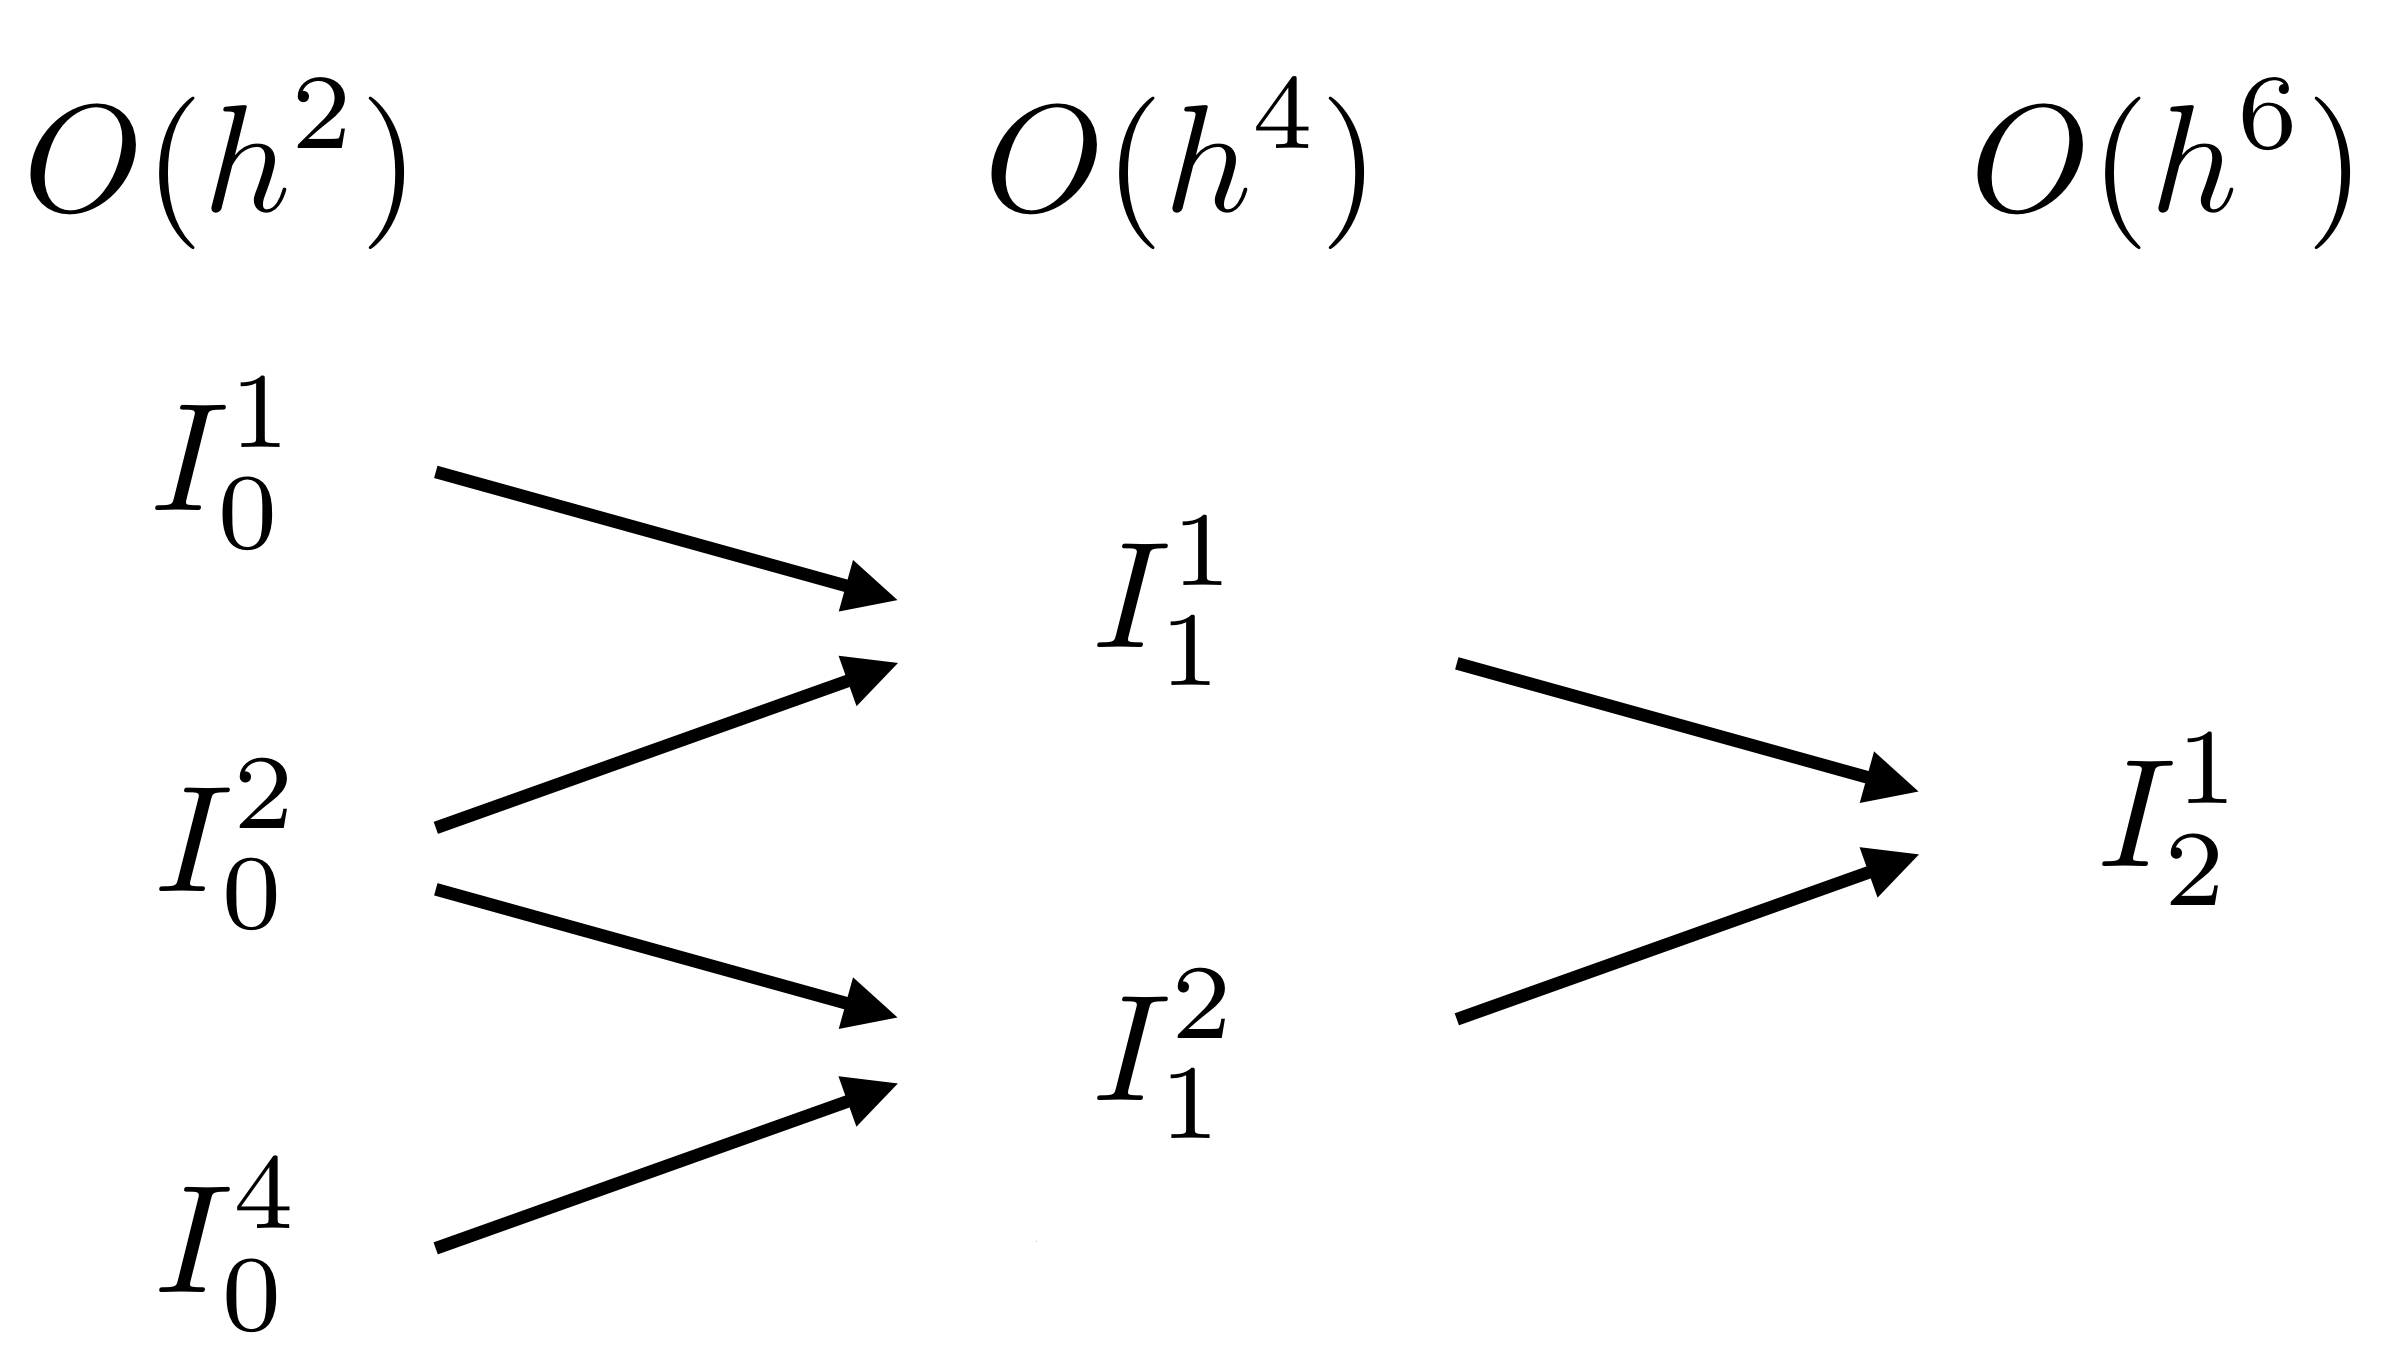
\includegraphics[width = 0.35\linewidth]{images/04/Romberg.jpeg}
        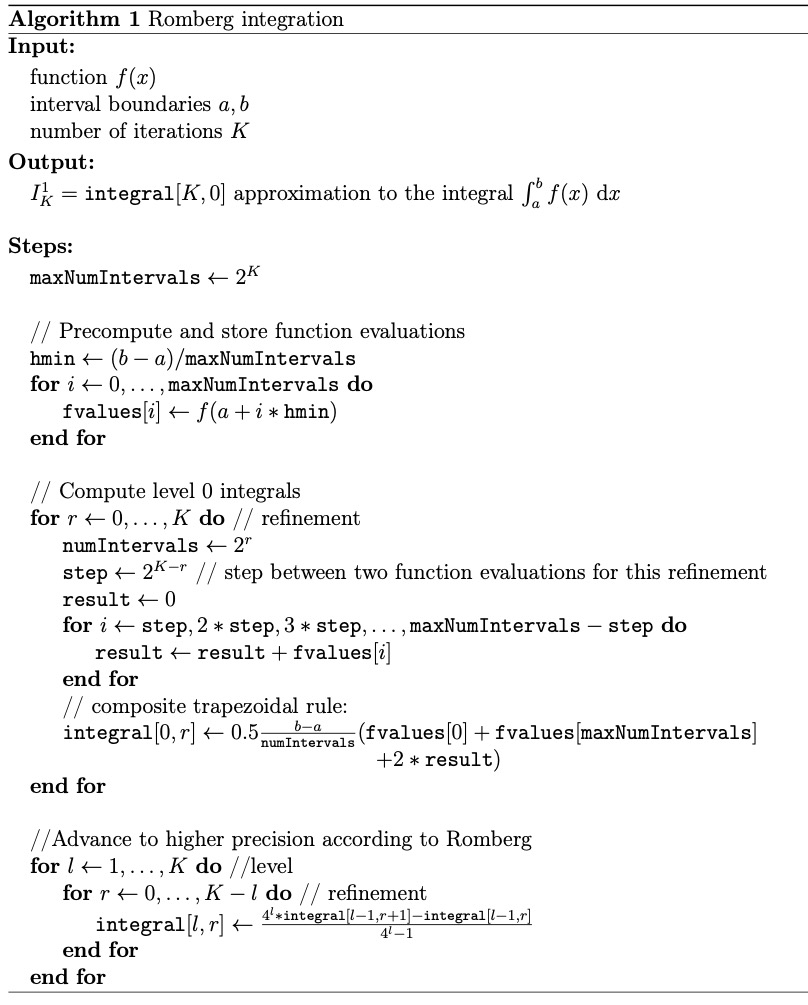
\includegraphics[width = \linewidth, height = 7.84cm]{images/04/Romberg_pseudo.jpg}
    \end{center}
    \subsection{Adaptive Quadrature}
    Romberg may achieve arbitrary accuracy but is not very efficient (function evaluations). Irregular function may waste evaluatins in flat regions.
    
    \begin{center}
        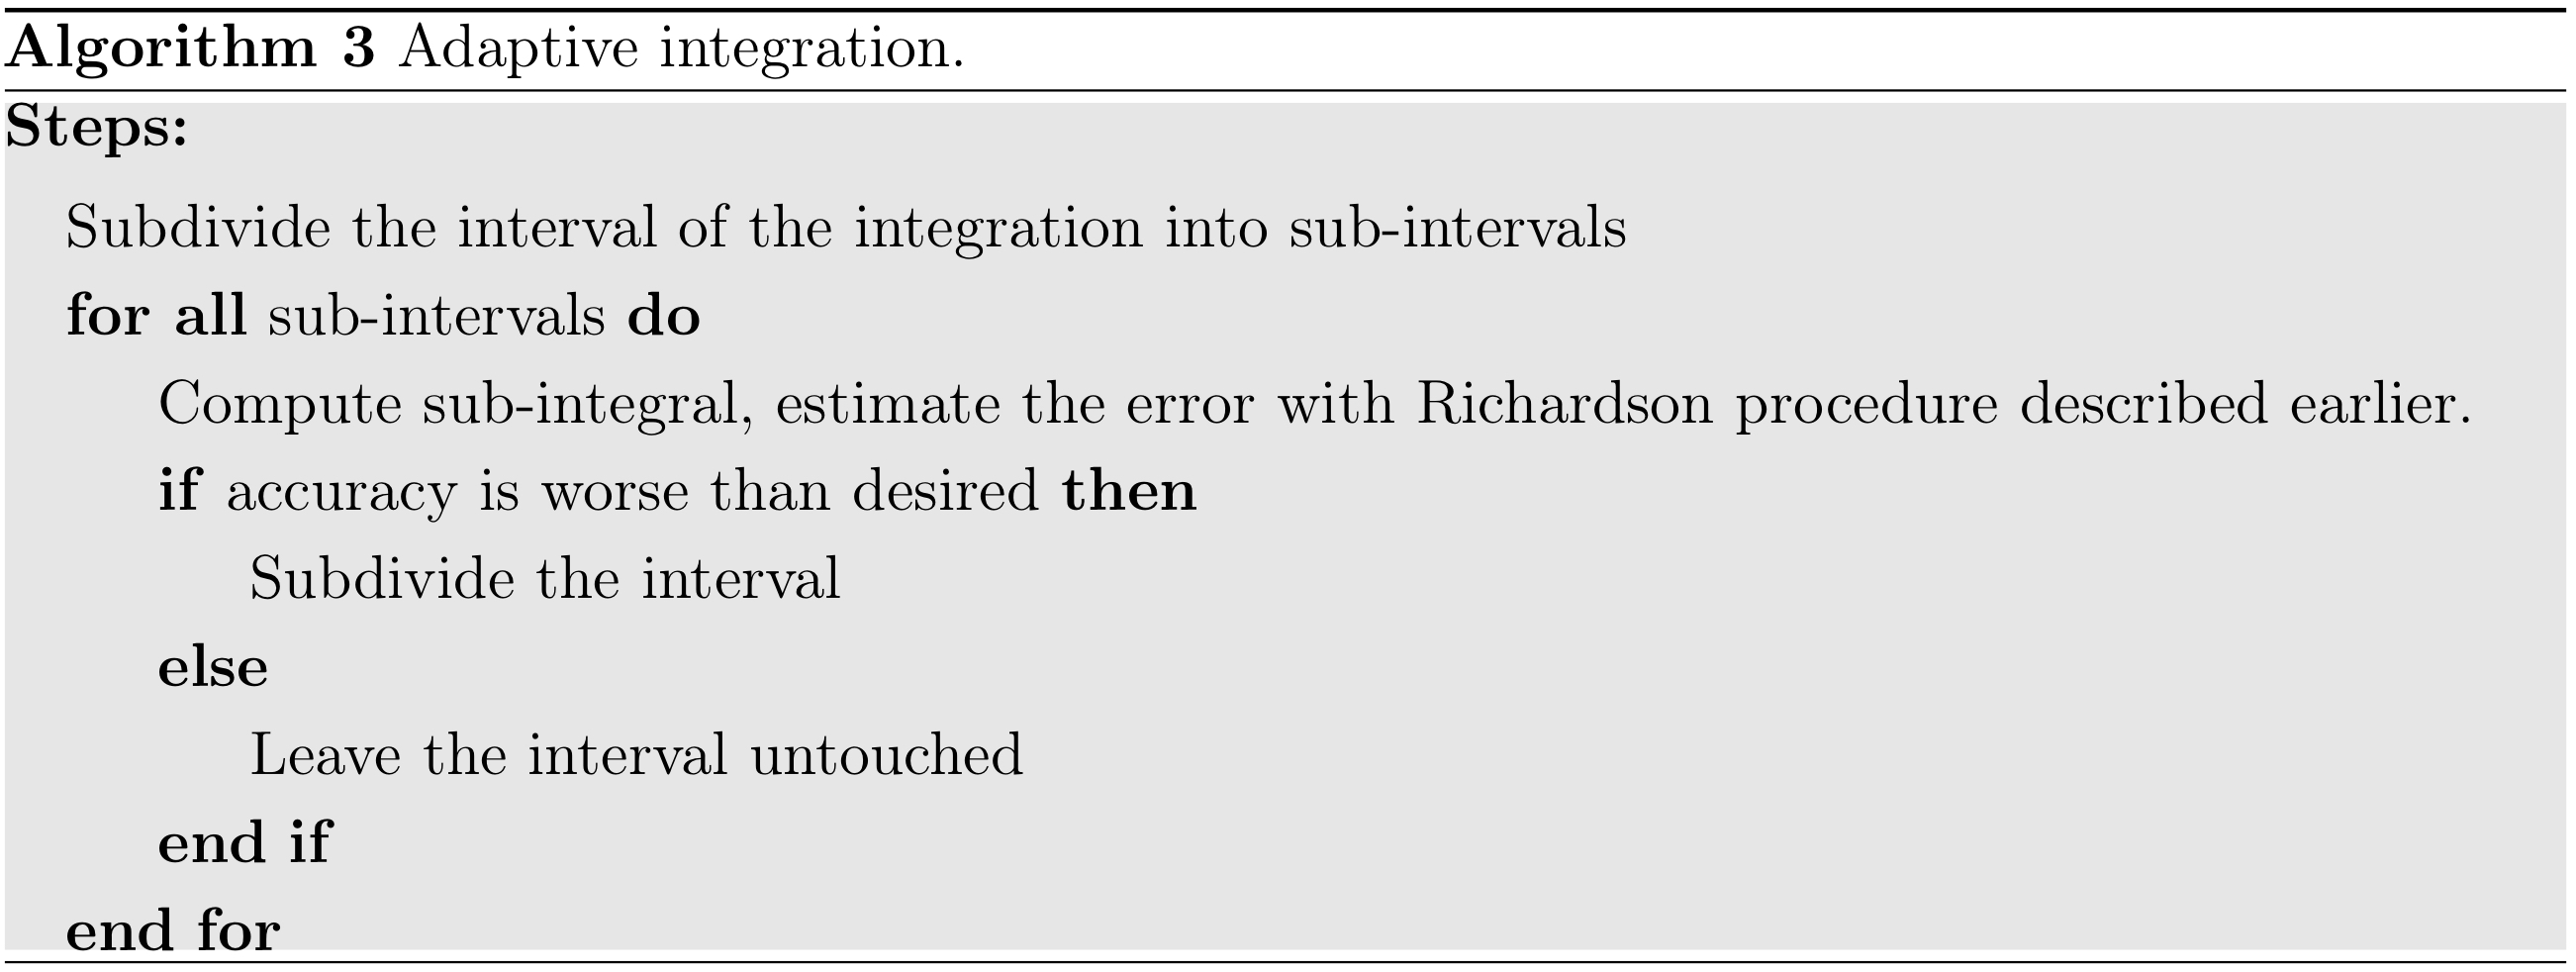
\includegraphics[width = \linewidth]{images/04/adaptive_quad.jpeg}
    \end{center}
    
\subsection{Gauss Quadrature}
   We adapt the weights and abscissas of our quadrature rule to obtain better accuracy.
    
    \subsubsection{Two-Point Gauss Quadrature}
        The two point gauss quadrature rule approximates $I$ using
        \begin{equation*}
            I = \int_a^b f(x)dx \approx c_1 f(x_1) + c_2 f(x_2)
        \end{equation*}
        where $c_1, \,c_2, \, x_1$ and $x_2$ are unknowns. They are evaluated by requiring an exact fit for an arbitrary third degree polynomial. Solving the nonlinear system of equations yields the two-point Gauss Quadrature rule:
        
        \begin{equation*}
            \colorboxed{red}{
            \begin{aligned}
            I \approx \frac{b-a}{2}\cdot f \left[\left(\frac{b-a}{2}\right)\left(\frac{-1}{\sqrt{3}}\right) + \frac{b+a}{2}\right]\\ +  \frac{b-a}{2}\cdot f\left[ \left(\frac{b-a}{2}\right)\left(\frac{1}{\sqrt{3}}\right) + \frac{b+a}{2}\right]
            \end{aligned}
            }
        \end{equation*}
    \subsubsection{\textit{n}-Point Gauss Quadrature}
        Goal: integrate $\int_a^b f(x)dx$.
        \begin{itemize}
            \item First we need to change the area of integration from $(a,b)$ with variable $\xi$ to $(-1,1)$ with variable $x$.
                \begin{equation*}
                    \colorboxed{red}{
                    x = \frac{2\xi - (a+b)}{b-a}
                    }
                \end{equation*}
                $I = \int_{-1}^1\frac{b-a}{2}f\left(\frac{b-a}{2}(z - 1) +b\right)dz$
            \item The integration points $x_i$ and the corresponding weights $w_i$ can be read from a table.
            
            \item the Integral is then evaluated using
            \begin{equation*}
            \colorboxed{red}{
                I \approx \frac{b-a}{2}\sum_{i=1}^n w_i f\left(\frac{b-a}{2}(z_i - 1) +b\right)
                }
            \end{equation*}
            
            \item Error with $n$ abscissas:
            \begin{equation*}
            \colorboxed{red}{
                \varepsilon = \frac{2^{2n+1}(n!)^4}{(2n+1)(2n!)^3}f^{(2n)}(\xi)
                }
            \end{equation*}
        \end{itemize}
        Gauss Quadrature gives the best accuracy, in the sense of correctly integrating polynomials of highest possible order for a given number of function evaluations. The Abscissas vary from order to order resulting in new evaluations of the abscissas from scratch if the accuracy of the Quadrture is to be imporved.
        
        the abscissas are the zeros of the Legendre polynomial of degree $n$.
        
       
    \subsection{Quadrature in multiple dimensions}
    \textbf{Goal:} Integrate $f:\mathbb{R}^d\to\mathbb{R}$ over a multi-dimensional domain $\Omega = \Omega_1\times\dots\Omega_d$ i.e. $ I = \int_\Omega fd\vec{x}$
    \begin{align*}
         I \overset{\substack{\textnormal{Fubinis}\\\textnormal{theorem}}}{=}&\int_{\Omega}\dots\int_{\Omega_d}f(x^{(1)},\dots,x^{(d)})dx^{(d)}\dots dx^{(1)}\\
         \approx &\sum_{i_1=1}^{N_1}\dots\sum_{i_d=1}^{N_d} \underbrace{w_{i_1}\dots w_{i_N}}_{= \underline{\underline{W}}_{i_1,\dots,i_d}} f(x_{i_1},\dots, x_{i_D})
    \end{align*}
    $\underline{\underline{W}} = \Vec{w}\Vec{w}^\top$ where $\Vec{w}$ is the $N\times 1$ dimensional weight vector as specififed by section \ref{sssec:totalint}
    
    \subsection{Curse of Dimensionality}
    Integrating in multiple dimensions leads to a rapid decrease in accuracy with increasing number of dimensions. The quadrature rules in \ref{ss:intrules} become of order $\colorboxed{red}{\mathcal{O}(M^{-s/d})}$ where $s$ is the order over a whole domain in 1 dimension and $d$ corresponds to the dimensionality of the Integration with total number of quadrature points $M$.

\subsection{Probability}
    Probability that $x\in(a,b)$ in a PDF:
    \begin{equation*}
        P(a\leq X \leq b) = \int_a^b p(x)dx
    \end{equation*}
    
    Uniform distribution $\mathcal{U}([a,b])$ and Normal distribution $\mathcal{N}(\mu, \sigma^2)$:
    \begin{gather*}
        p_{\mathcal{U}}(x) = 
        \begin{cases}
            \frac{1}{b-a} &x\in(a,b)\\
            0 &\textnormal{otherwise}
        \end{cases}\\
        p_{\mathcal{N}} = \frac{1}{\sqrt{2\pi\sigma^2}}\exp\left( -\frac{(x-\mu)^2}{2\sigma^2}\right)
    \end{gather*}
    
    Expected value $\mathbb{E}$ over a domain $\Omega$:
    \begin{gather*}
        \mathbb{E}[X] = \langle X \rangle = \int_\Omega xp(x)dx \quad (=\mu \textnormal{ mean})\\
        \mathbb{E}[h(x)] = \int_\Omega h(x)p(x)dx
    \end{gather*}
        % $\mathbb{E}[aX+bY] = a\mathbb{E}[X] + b\mathbb{E}[Y]$
        \\Discrete form: $\mathbb{E}[X] = \Bar{x} = \sum_i x_iP(x_i)$
    
    Variance:
        \begin{equation*}
            \textnormal{Var}[X] = \sigma^2[X] = \mathbb{E}[X^2]- \mathbb{E}[X]^2
        \end{equation*}
    
    \subsubsection{Inverse Transform Sampling}
        Solve for u. We can thus sample any distribution from a uniform distribution.
        \begin{equation*}
            F(x) = \int_0^x p(x)dx = u
        \end{equation*}
    
    \subsubsection{Rejection Sampling}
        Generate samples from $p(x)$ from a simple distribution function $h(x)$ from which we already know how to generate samples. $h(x)$ has to bound $p(x)$. $p(x) < \lambda p(x)$
        \begin{enumerate}
            \item draw random sample $x$ for $h(x)$
            \item draw uniform random number $u\in[0,1]$
            \item accept $x$ if $x < \frac{p(x)}{\lambda h(x)}$, else reject $x$
        \end{enumerate}
    
    \subsubsection{Importance Sampling}
        ``Bad" fitting $h(x)$ might waste a lot of evaluations. We want to draw samples $x$ from probability $w(x)$ which fits better. We compensate for the bias by nomralizing $p(x)$ by $w(x)$ and thus sample $p(x)/w(x)$.
        \begin{equation*}
            \langle f \rangle_p = \int_a^b f(x)\frac{p(x)}{w(x)}w(x)dx \approx \frac{1}{M}\sum_{i=1}^M f(x_i)\frac{p(x_i)}{w(x_i)}
        \end{equation*}
        With each $x_i$ being sampled from distribution $w(x)$.
    
\subsection{Monte Carlo}
    \textbf{Recipe:}
    \begin{enumerate}
        \item Sample points $\Vec{x}_i$ from a uniform distribution and evalutate inegrand $f$ to get $f(\Vec{x}_i)$.
        
        \item Store number of samples, the sum of the values and the sum of squares
        \begin{equation*}
            M, \quad \sum_{i=1}^M f(\Vec{x}_i), \quad \sum_{i=1}^M f(\Vec{x}_i)^2
        \end{equation*}
\vspace{-2mm}       
        \item Compute mean as the estimate of the expectation (\textbf{normalized integral})
        \begin{equation*}
            \frac{I}{|\Omega|} = \langle f \rangle \approx \langle f \rangle_M = \frac{1}{M}\sum_{i=1}^M f(\Vec{x}_i)
        \end{equation*}
\vspace{-2mm}        
        \item Estimate the variance using the unbiased sample variance:
        \begin{equation*}
            \textnormal{Var}[f] \approx \frac{M}{M-1}\left(\frac{1}{M}\sum_{i=1}^M f(\Vec{x}_i)^2-\langle f \rangle_M\right)
        \end{equation*}
\vspace{-2mm}       
        \item estimate error
        \begin{equation*}
            \varepsilon_M = \sqrt{\frac{\textnormal{Var}[f]}{M}}
        \end{equation*}
    \end{enumerate}
    

\section{Neural Networks}
    Function $\y(\cdot,\w): \mathbb{R}^{n_0}\rightarrow\mathbb{R}^{n_L}$ parametrized by weights $\w$.

\subsection{2-Layer NN}
    Notation for weights is $w_{ji}^\ell$ with destination node $j$ and source node $i$ in layer level $\ell$. We denote the input of the layer $\ell$ and node $j$ as $a_j^\ell$.
    Define Matrix $W^\ell$ with $W_{ij}^\ell = w_{ij}^\ell$. Activation function acts elementwise on the vectors.
    \begin{equation*}
        \y(\Vec{x};\w) = \p_2\bigg(W^2\p_1\Big(W^1\Vec{x}\Big)\bigg)
    \end{equation*}
\subsection{\textit{L}-layer NN}
    The contents of the previous section can be generalized for an arbitrary amount of intermediate layers.
     \begin{center}
            \renewcommand{\arraystretch}{1.3}{\begin{tabular}{l|c}
                Input $\ell^{th}$ layer & $\displaystyle a_j^\ell = \sum_{i=0}^{n_0} w_{ji}^\ell z_i^{\ell - 1}$\\
                Output $\ell^{th}$ layer & $\displaystyle z_j^\ell = \p_{\ell}(a_j^\ell)$
            \end{tabular}}
    \end{center}
    \begin{equation*}
        \y(\Vec{x};\w) = \p_L\Bigg(W^L\p_{L-1}\Big(\dots W^2\p_2\big(W^1\Vec{x}\big)\Big)\Bigg)
    \end{equation*}

\subsection{Activation Function}
    Ex: Heaviside Step, ReLU, tanh, logistic (sigmoid),...
    
    Introduce nonlinearity into the NN. Otherwise, the output of the NN would solely be a lin. comb. of the inputs. Smooth funcitons are preferred since they are differentiable (needed for backporpagation)
    

    \subsection{Backpropagation}
    \subsubsection{Learning}
        We want to minimize error function 
        \begin{equation*}
            E_n = \frac{1}{2}|\hat{\y}_n - \y(\Vec{x}_n,\w)|^2 \Rightarrow
            E(\w) = \sum_{n=1}^N E_n(\w)
        \end{equation*}
        With data $\{\Vec{x}_n, \hat{\y}_n\}, \, n = 1,\dots,N$ and $\w = \{W^1,\dots,W^L\}$. We want to find $\w^\star=\arg\min E(\w)$ using gradient descent \Big(stochastic gradient descent: Change $E(\w^{(k)})$ to $E_n(\w^{(k)})$/batchSGD: Change $E(\w^{(k)})$ to $\sum_{n\in\mathcal{I}}E_n(\w^{(k)})$\Big).
        \begin{equation*}
            \w^{(k+1)} =\w^{(k)} - \eta\nabla_{\w}E(\w^{(k)})
        \end{equation*}
        
    \subsubsection{Backpropagation}
        Minimizing $E$ by computing the derivative w.r.t $w_{ji}^\ell$ using chain rule.
        \begin{equation*}
            \frac{\partial E_n}{\partial w_{ji}}= \frac{\partial E_n}{\partial a_j}\frac{\partial a_j}{\partial w_{ji}} = \delta_j \Tilde{\Tilde{z}}_i = \p'(a_j)\sum_k \Tilde{w}_{kj}\Tilde{\delta}_k \cdot \Tilde{\Tilde{z}}_i
        \end{equation*}
        with the output of the previous node $\Tilde{\Tilde{z}}_i$. Computation of $\delta_j$ depends on $\Tilde{\delta}_k$ (i.e. on the layer on its right. for the last layer $\delta_j = y_j(\Vec{x}_n; \w) - \hat{y}_{nj}$.
    
\subsection{Overfitting}
    A model with $N$ free parameters should be able to fit exactly $N$ data points. However, if the model passes exactly through the points it is unlikely to generalize efficiently since it fits the behaviour of noise. But if too few parameters are used, the model might be forced to ignore meaningful data. \textbf{Bias-Variance Trade-off}
    
\section{Dimensionality Reduction}
    \subsection{Principal Component Analysis}
    Linear transformation onto a subspace explaining the most variance (minimize reconstruction loss). Given dataset $X^\top = (\Vec{x}_1,\dots,\Vec{x}_N)\in\mathbb{R}^{D\times N}$ with $N$ Vectors of $D$ elements $\Vec{x}_n\in\mathbb{R}^D,\, n = 1,2,\dots,N$. %We assume zero mean.
    %Otherwise, we transfrom data, such that this property is satisfied:
    % \begin{gather*}
    %     \Tilde{\Vec{x}}_n = \Vec{x}_n - \bar{\Vec{x}},\quad \bar{\Vec{x}}=\frac{1}{N}\sum_{n=1}^N \Vec{x}_n\\
    %     C = \frac{1}{N-1}\Tilde{X}^\top\Tilde{X},\, C\in\mathbb{R}^{D\times D} 
    % \end{gather*}
    Solving for the first principal component (direction in $\Vec{v}_1^\star\in\mathbb{R}^D$ s.t. variance of projected data is maximized) yields ${\sigma_1^\star}^2 = \lambda_1^\star \rightarrow$ Maximum of objective function correspond to the EigVec of the max EigVal.
    
    \textbf{Recipe:}
    \begin{enumerate}
        \item Construct centered data matrix
            \begin{equation*}
                X^\top\in\mathbb{R}^{D\times N}
            \end{equation*}
            
        \item Construct Covariance Matrix 
            \begin{equation*}
                C = \frac{1}{N-1}X^\top X,\ C\in\mathbb{R}^{D\times D}
            \end{equation*}
        
        \item Perform eigenvector decomposition of C.
        \item Sort EigVec in decr. EigVal order $\lambda_1\geq\lambda_2\geq\dots\geq\lambda_D$ to construct $V_r = (\Vec{v}_1,\dots,\Vec{v}_r)\in\mathbb{R}^{D\times r}$ for the transformation 
        \begin{equation*}
        Y_r = V_r^\top X^\top, \quad Y_r \in\mathbb{R}^{r\times N}
        \end{equation*}
        
        \item \Big(Reconstruction: $\Tilde{X} = X V_r V_r^\top$\Big)
        
    \end{enumerate}
    
    Percentage of retained variance:
    \begin{equation*}
        \textnormal{ratio} = \frac{\sum_{i=1}^r \lambda_i}{\sum_{i=1}^D \lambda_i}
    \end{equation*}
\end{multicols*}     

\end{document}